\chapter{Measurements from IMU}\label{app:IMUMeasurementsAppendix}
\textbf{Name: Group 630}\\
\textbf{Date: 2/05 - 2016}

\subsubsection{Purpose}
Get data from the IMU and the potentiometer when running the state-space controller, and used it to design the complementary filter.             

\subsubsection{List of Equipment}
\begin{table}[H]
	\begin{tabular}{|l|l|p{4.3cm}|}
		\hline%------------------------------------------------------------------------------------
		\textbf{Instrument}                        &  \textbf{AAU-no.}  &  \textbf{Type}       \\
		\hline%------------------------------------------------------------------------------------
		Cubli setup                              &               &  		  \\
		\hline%------------------------------------------------------------------------------------
		Dedicated Power Supply of Cubli \small{(24 V - 3 A)} &               &  XP Power, AEB70US24 \\
		\hline%------------------------------------------------------------------------------------
		Computer                &              &  Asus A55V          \\
		\hline%------------------------------------------------------------------------------------
	\end{tabular}
\end{table}
\subsubsection{Procedure}
\begin{enumerate}
	  \item Plug the power supply given with the Cubli setup to a \si{220}{V} power outlet.
	  \item Wait until the blue LEDs on the Beaglebone Black start blinking slowly and connect the USB cable to the PC.
	  \item Send the binary compiled program of the controller to the board.
	  \item Connect to a distant terminal on the Beaglebone Black through SSH and launch the program.
	  \item Let the program run with the state-space controller.
	  \item Apply small disturbances to the Cubli so there is some variations in the angle
	  \item Stop the program (by pressing \textit{Q} and \textit{ENTER}).
	  \item Retrieve the log file from the Cubli setup with the recorded data.
\end{enumerate}

\subsubsection{Results}
%The measured data is partially converted through the code. Accelerometer and gyro values are given in rad/s. \fxnote{might need changing if we have to redo the conversion, B}
%Data from the accelerometer is converted into an angle with arctan and the gyro data is integrated because the gyroscope is measuring the angular velocity in the direction of the frames rotation. This is done to see how close the potentiometer the angle the data comes.
%The data is available as a .csv file on the CD\fxnote{Make sure this is put into the CD folder for copying}
%
%To find the angle from the accelerometer data is done the following equation:
%\begin{flalign}
%	&\si{\theta_{F}=\arctan(\frac{y_1}{x_1})}&
%	\label{eq:accelToAngle}
%\end{flalign}
%
%The gyroscopes angular velocity measurement is integrated.
%The integration is done the same way it would be done in the code on the BeagleBone.
%\begin{flalign}
%	&\si{\theta_{F}[n]=\theta_{F}[n-1]+\omega[n] \cdot \Delta T}&
%	\label{eq:gyroToAngle}
%\end{flalign}
%
%\si{\Delta T} being the samplingfrequency of the controller.

\begin{figure}[H]
	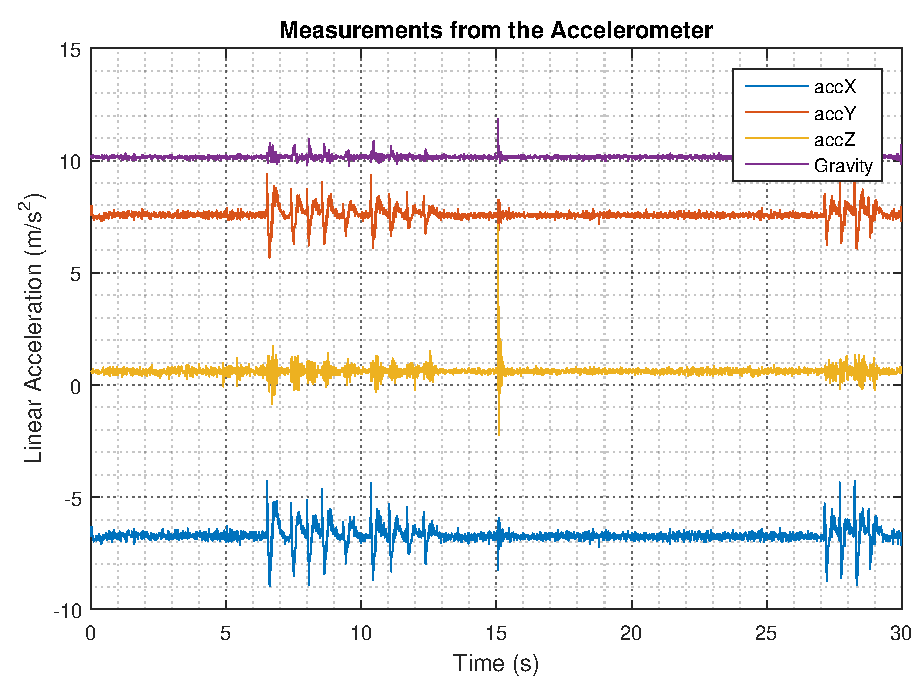
\includegraphics[scale=.75]{figures/accData}
	\centering
	\caption{Linear acceleration measurements from the accelerometer and the calculated gravity magnitude}
\end{figure} \label{accData}
%
\begin{figure}[H]
	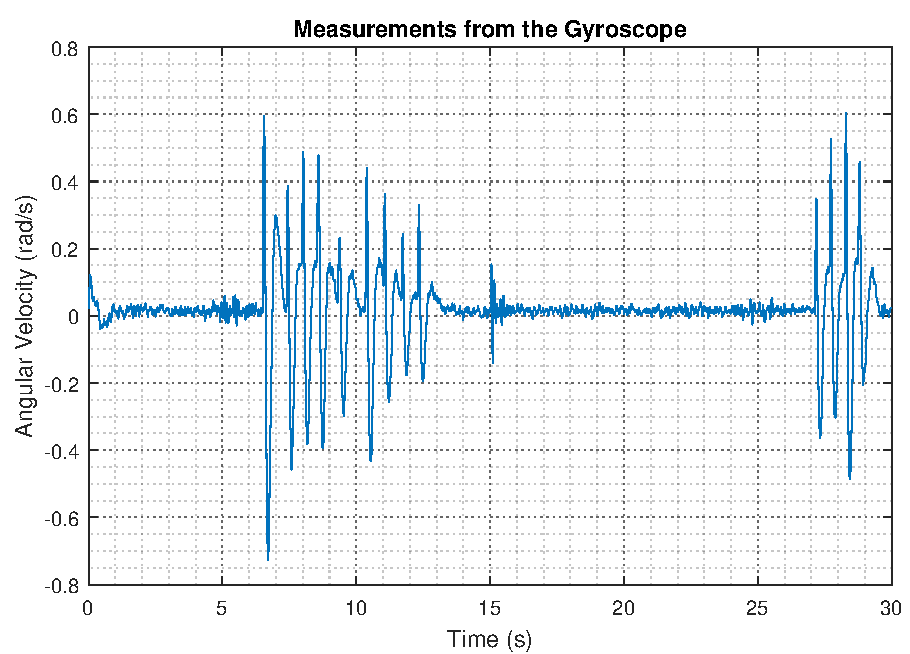
\includegraphics[scale=.75]{figures/gyroData}
	\centering
	\caption{Angular velocity measurements from the gyroscope}
\end{figure} \label{gyroData}
%
\begin{figure}[H]
	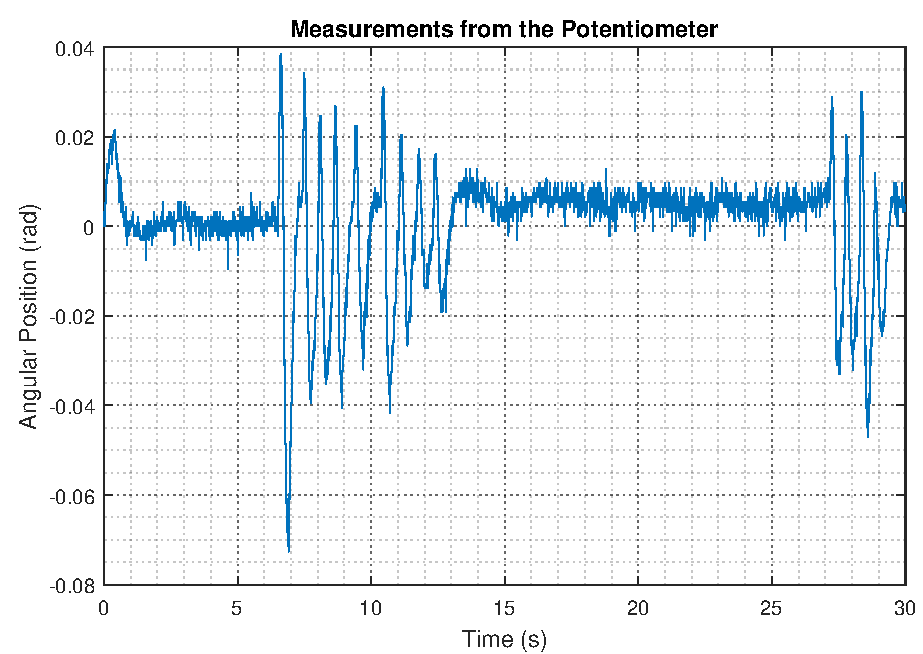
\includegraphics[scale=.75]{figures/potData}
	\centering
	\caption{Angle measurements from the potentiometer}
\end{figure} \label{potData}
